\documentclass[english,11pt]{beamer}

\DeclareMathOperator{\Cov}{Cov}
\DeclareMathOperator{\Var}{Var}
\DeclareMathOperator{\E}{\mathbb{E}}
\DeclareMathOperator{\Proba}{\mathbb{P}}

\newcommand{\Covb}[2]{\ensuremath{\Cov\!\left[#1,#2\right]}}
\newcommand{\Eb}[1]{\ensuremath{\E\!\left[#1\right]}}
\newcommand{\Pb}[1]{\ensuremath{\Proba\!\left[#1\right]}}
\newcommand{\Varb}[1]{\ensuremath{\Var\!\left[#1\right]}}

% norm
\newcommand{\norm}[1]{\| #1 \|}

\newcommand{\indep}{\rotatebox[origin=c]{90}{$\models$}}





\usepackage{mathptmx,amsmath,amssymb,graphicx,bibentry,bbm,babel,ragged2e}

\makeatletter

\newcommand{\noun}[1]{\textsc{#1}}
\newcommand{\jitem}[1]{\item \begin{justify} #1 \end{justify} \vfill{}}
\newcommand{\sframe}[2]{\frame{\frametitle{#1} #2}}

\newenvironment{centercolumns}{\begin{columns}[c]}{\end{columns}}
%\newenvironment{jitem}{\begin{justify}\begin{itemize}}{\end{itemize}\end{justify}}

\usetheme{Warsaw}
\setbeamertemplate{footline}[text line]{}
\setbeamercolor{structure}{fg=purple!50!blue, bg=purple!50!blue}

\setbeamersize{text margin left=15pt,text margin right=15pt}

\setbeamercovered{transparent}


\@ifundefined{showcaptionsetup}{}{%
 \PassOptionsToPackage{caption=false}{subfig}}
\usepackage{subfig}

\usepackage[utf8]{inputenc}
\usepackage[T1]{fontenc}



\makeatother

\begin{document}


\title{Towards Integrative Theories for Territorial Systems}

\author{J.~Raimbault$^{1,2,\ast}$\\
\texttt{juste.raimbault@polytechnique.edu}
}


\institute{$^{1}$UMR CNRS 8504 G{\'e}ographie-cit{\'e}s\\
$^{2}$UMR-T IFSTTAR 9403 LVMT
}

\date{}


\frame{\maketitle}


\sframe{Interactions between Networks and Territories}{

\centering

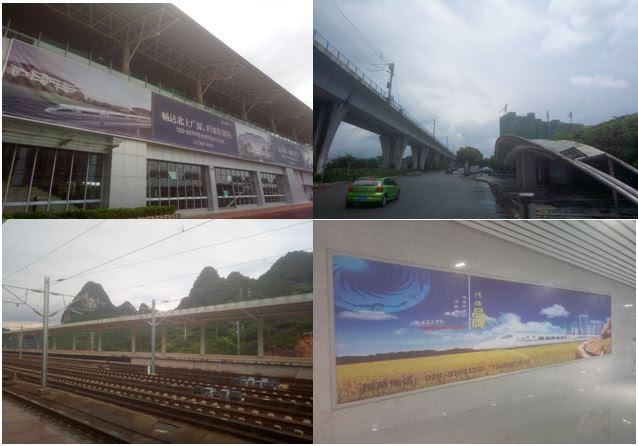
\includegraphics[width=0.9\textwidth]{figures/fieldwork}

\footnotesize

\textit{Fieldwork on High Speed Rail in China.}

}


\sframe{Modeling Urban Morphogenesis}{

\centering

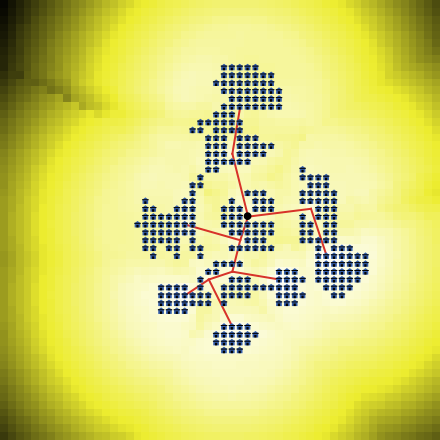
\includegraphics[width=0.46\textwidth]{figures/RBD_lattice}\hspace{0.1cm}
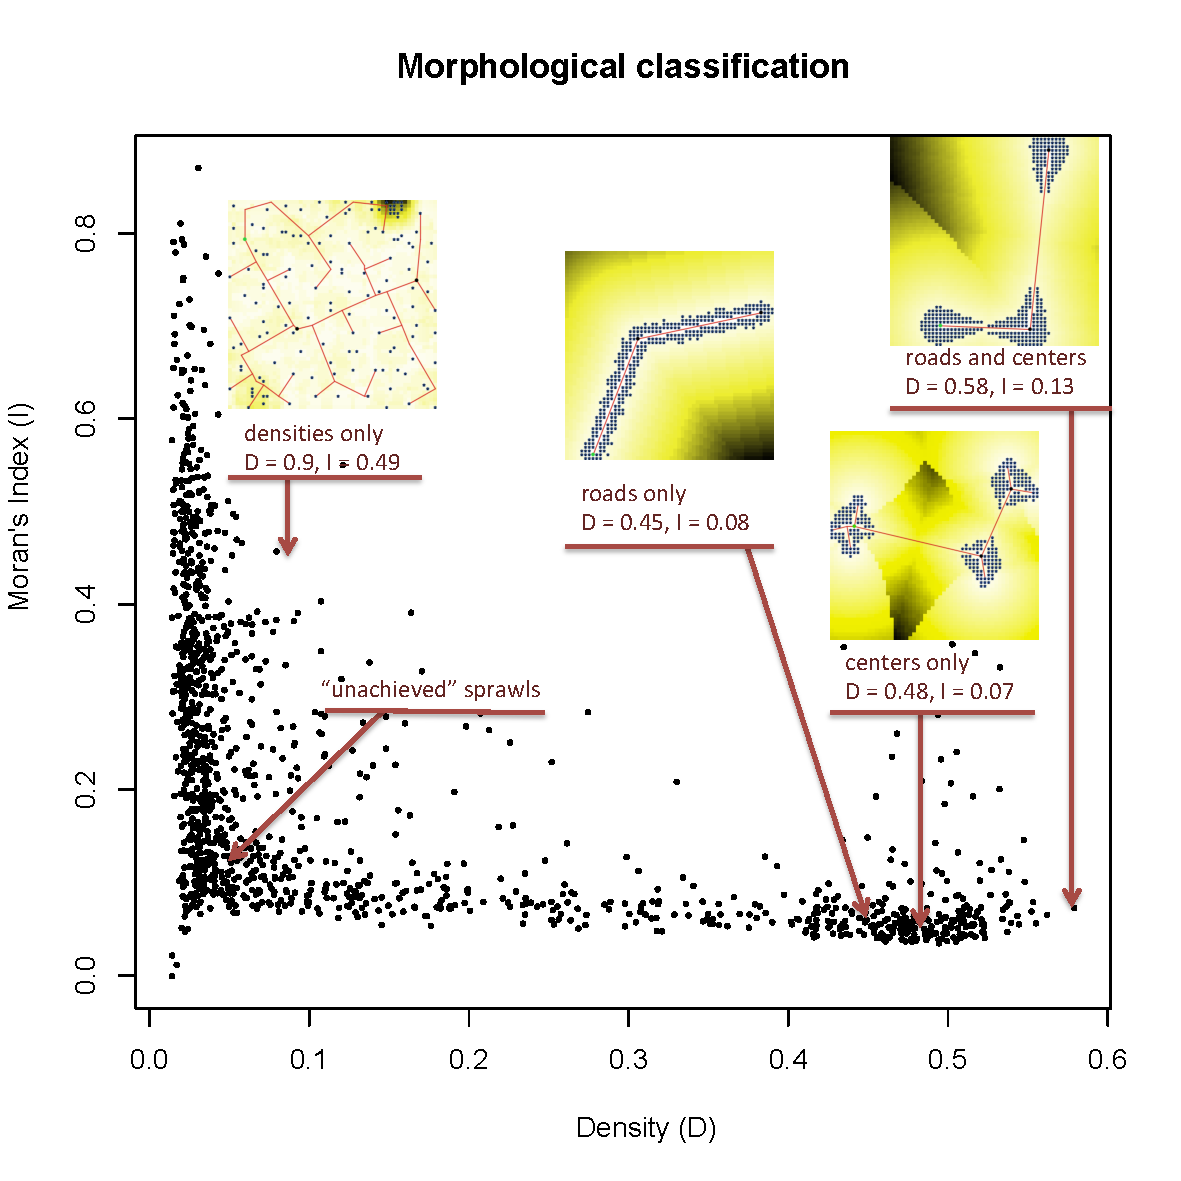
\includegraphics[width=0.51\textwidth]{figures/RBD_morpho}

\bigskip

\footnotesize
\textit{Raimbault, J., Banos, A., \& Doursat, R. (2014). A hybrid network/grid model of urban morphogenesis and optimization. ICCSA2014.}

}


\sframe{Non-equilibrium Micro-dynamics in Transportation Systems}{


\begin{columns}
\column{0.45\textwidth}
\centering
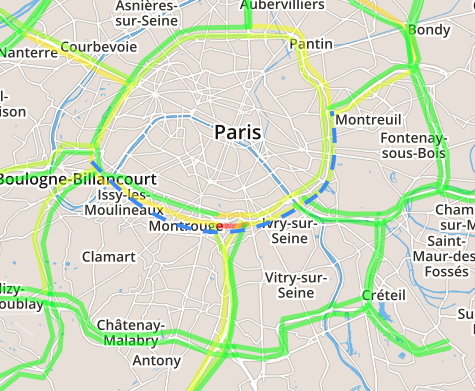
\includegraphics[width=0.65\textwidth]{figures/treq_gr21}\\\medskip
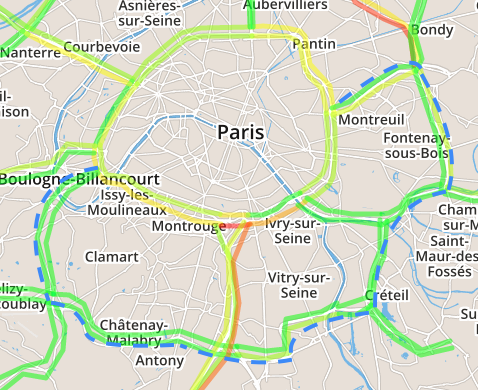
\includegraphics[width=0.65\textwidth]{figures/treq_gr22}

\column{0.55\textwidth}
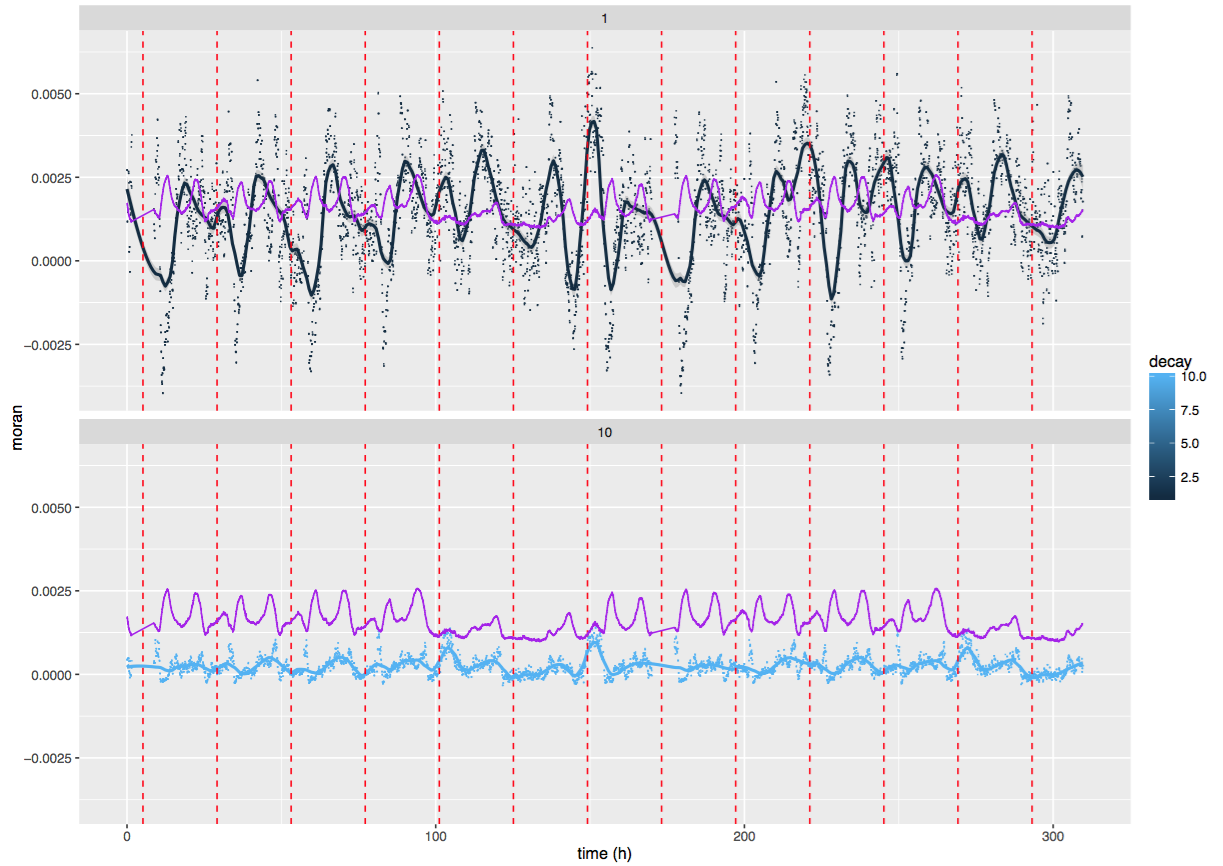
\includegraphics[width=\textwidth]{figures/treq_gr5}

\end{columns}

\bigskip

\centering

\footnotesize

\textit{Raimbault, J. (2017). Investigating the empirical existence of static user equilibrium. Transportation Research Procedia, 22, 450-458.}







}



\sframe{Processes of Knowledge Production}{

\centering

\includegraphics[width=0.35\textwidth]{figures/patents_Fig2}\hspace{0.1cm}
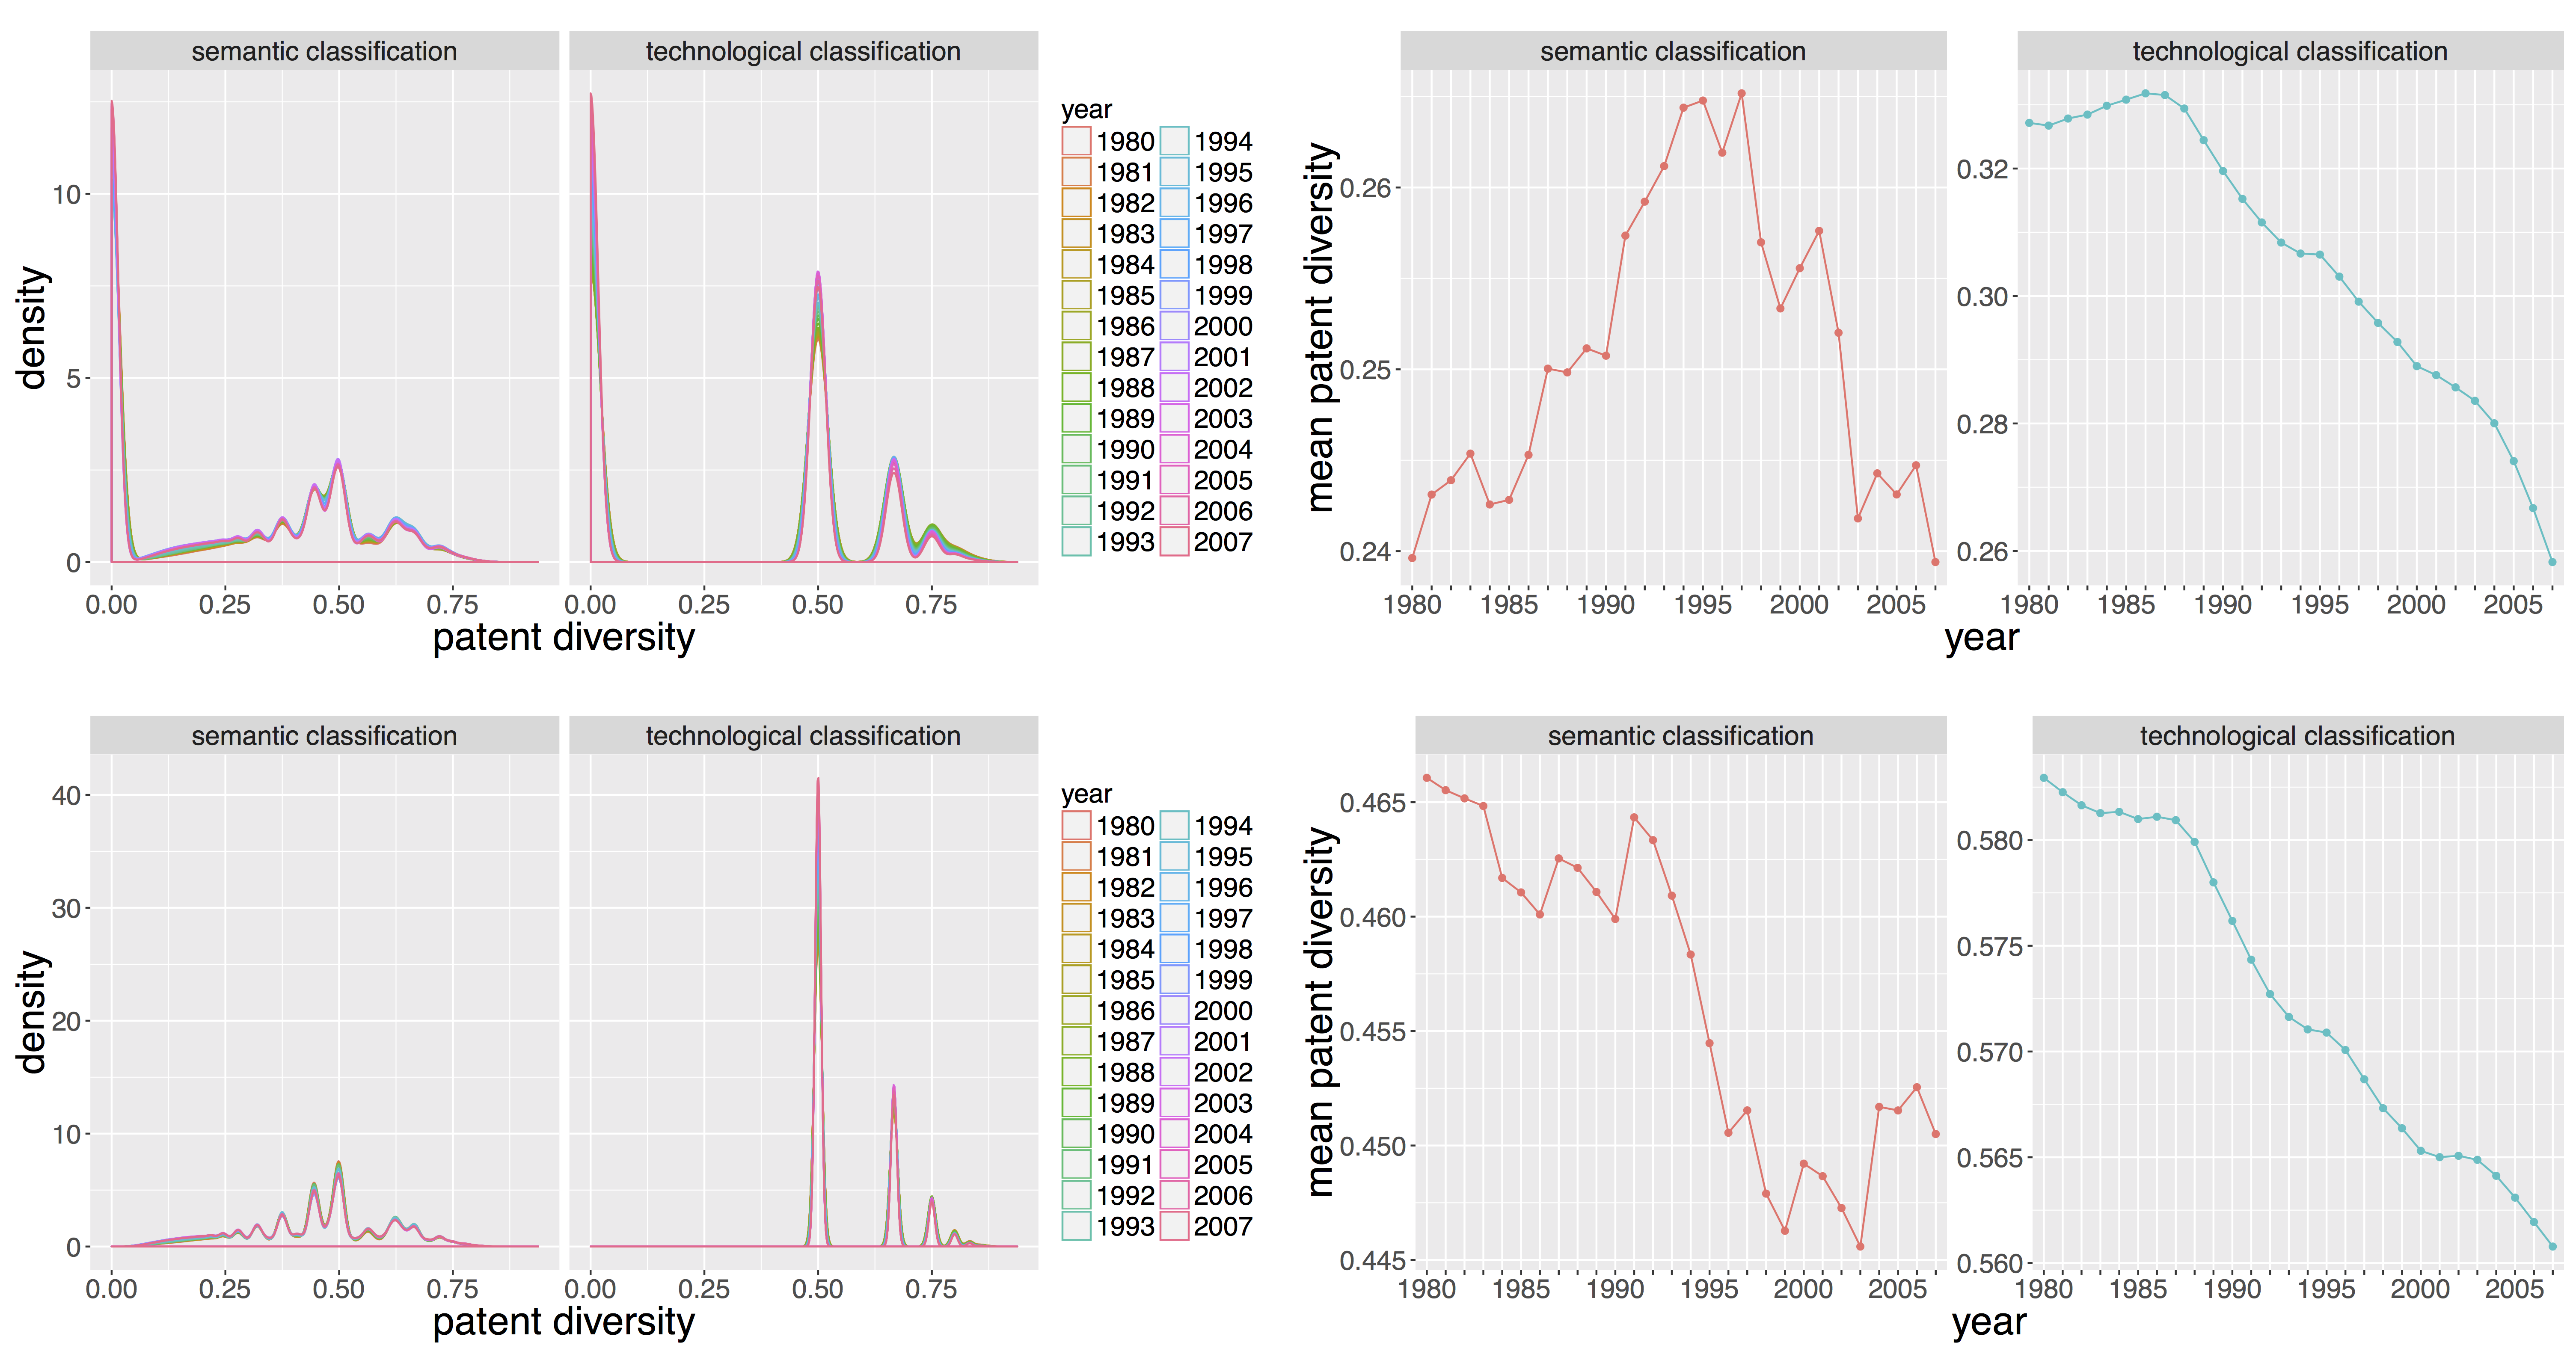
\includegraphics[width=0.6\textwidth]{figures/patents_Fig5}

\bigskip

\footnotesize
\textit{Bergeaud, A., Potiron, Y., \& Raimbault, J. (2017). Classifying patents based on their semantic content. PloS one, 12(4), e0176310.}

}



\sframe{Applied Epistemology}{

\centering

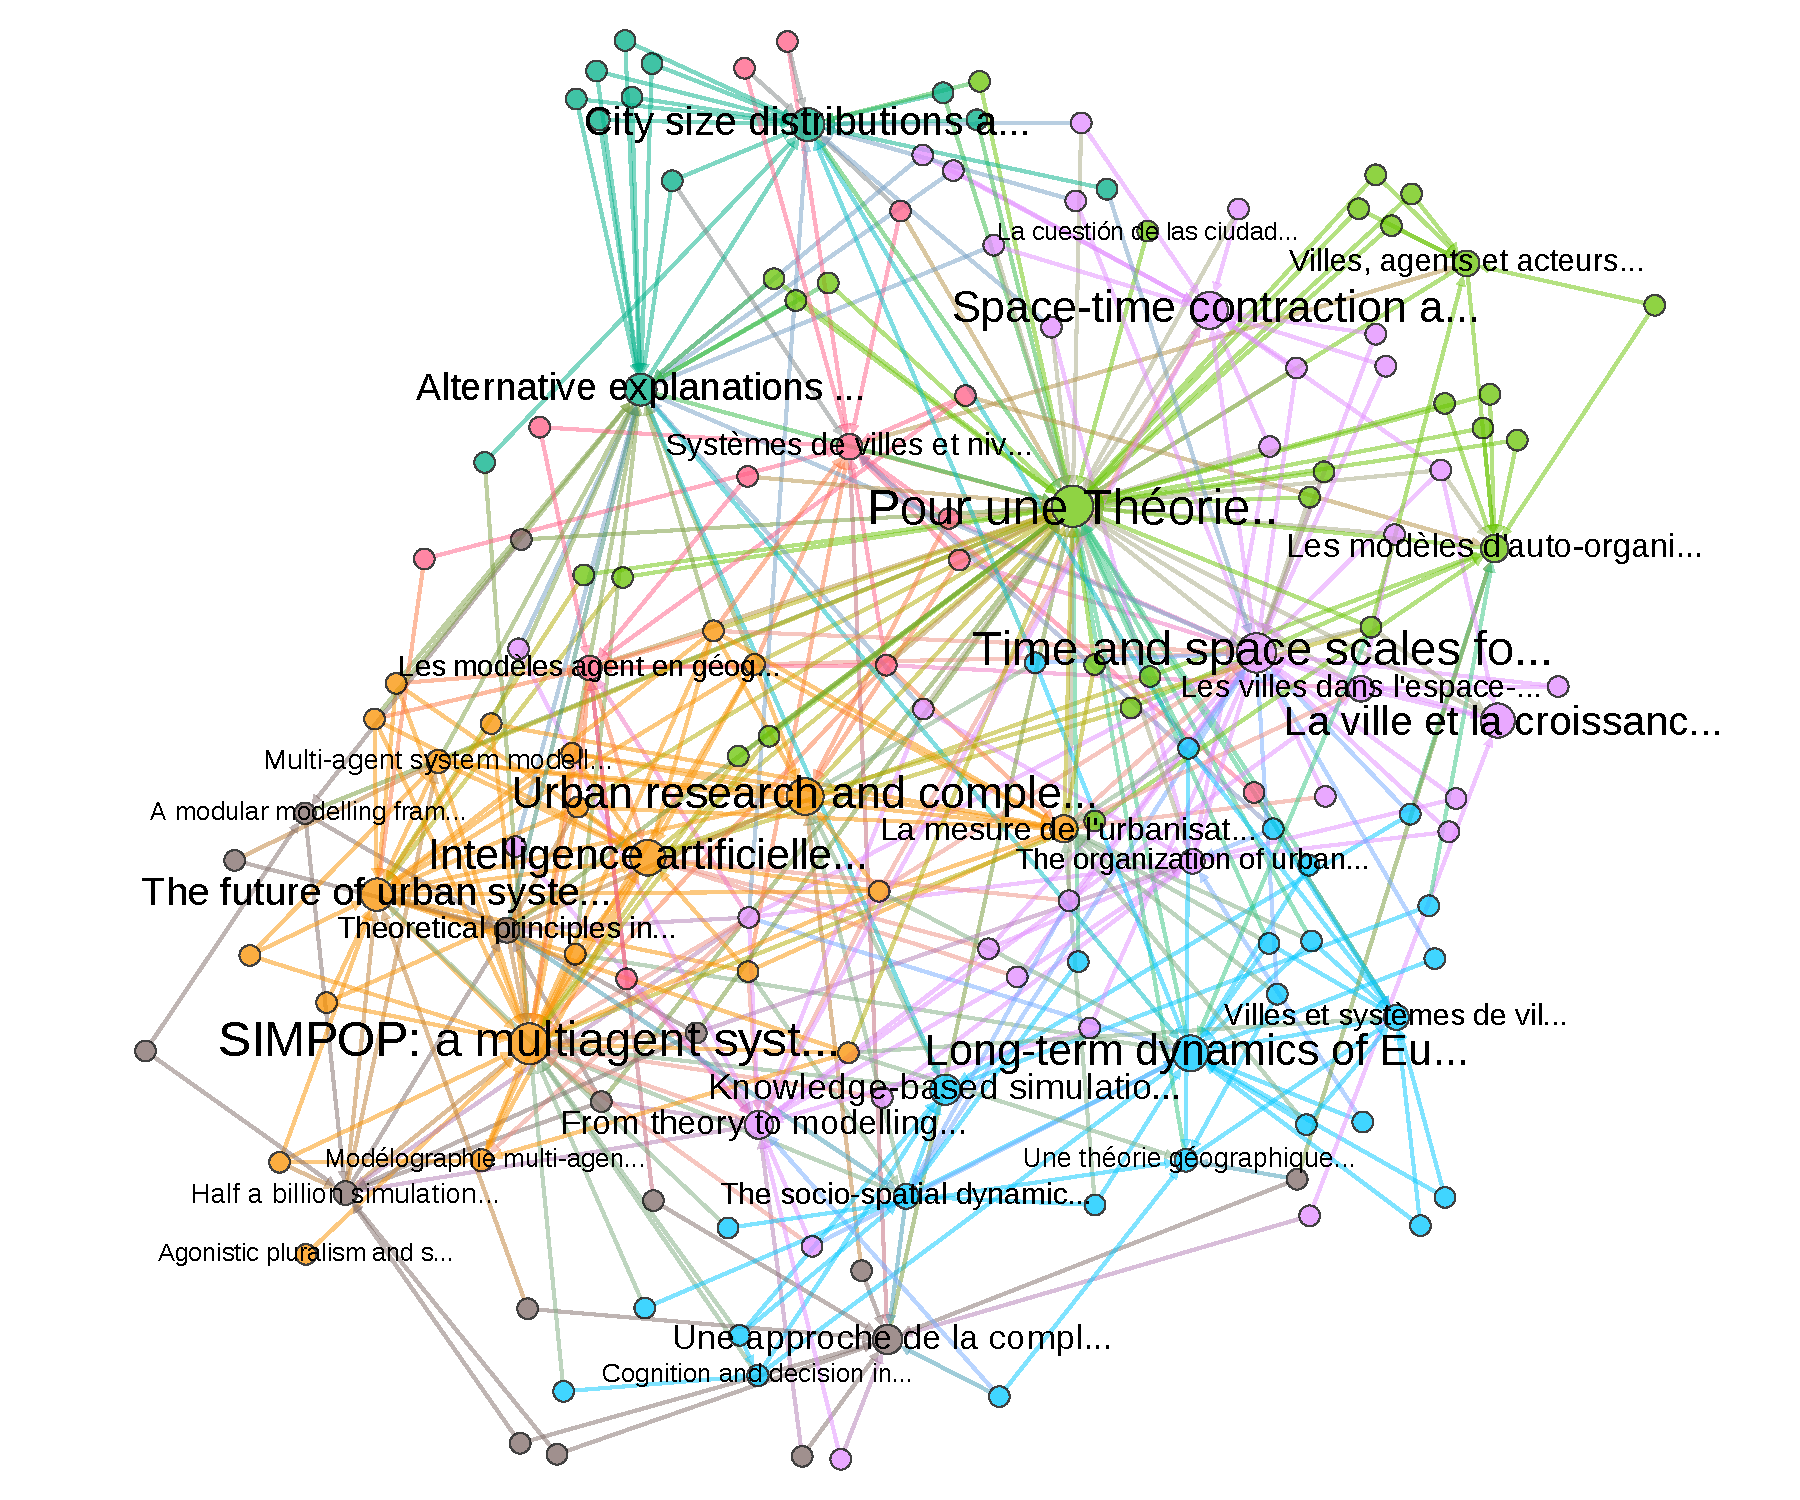
\includegraphics[width=0.48\textwidth]{figures/kf_core}\hspace{0.1cm}
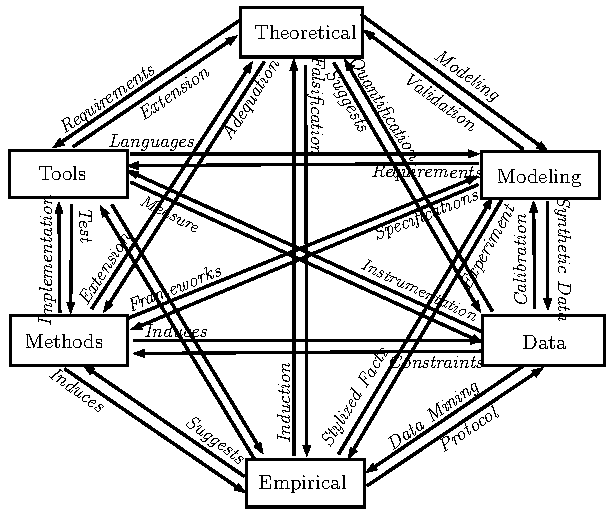
\includegraphics[width=0.48\textwidth]{figures/kf_framework}

\bigskip

\footnotesize
\textit{Raimbault, J. (2017). An Applied Knowledge Framework to Study Complex Systems. arXiv preprint arXiv:1706.09244.}

}





\end{document}







